% Author: David Sanchez-Jacome

\chapter{Universal Unitary Operators}\label{chap:universal_unitary_operators} % (fold)

Linear optical operations lie at the heart of several optical systems.
For example, optical hybrids are key components in Telecom coherent receivers \cite{faralli_compact_2015}, discrete Fourier transform (DFT) operators enable high-fidelity FMCW Lidar \cite{kim_fmcw_2020}, quantum information processing is performed using linear quantum logic gates \cite{arrazola_quantum_2021,harris_large-scale_2016}, signal processing in radar \cite{sanchez-jacome_coherent_2021} and multicore fiber systems \cite{sakamoto_strongly-coupled_2017} relies on the multiple-input and multiple-output (MIMO) technique to unscramble the signals and recover the information (i.e., a unitary matrix operation); among many other use cases \cite{carolan_universal_2015}.
Such operations are usually implemented by complex custom hardware systems that can't be reused for other applications.
Nevertheless, specific optical system architectures that can implement all these unitary operations on the same hardware are known to exist in bulk and integrated optics \cite{clements_optimal_2016}.
The feasibility studies to implement such unitary operations on programmable integrated platforms have gained significant attention and resources in the last decade.
It's expected that the solid-state nature of these devices will enhance the cost-efficiency, mass-manufacturability, and reusability of integrated unitary operators within several application fields.

In parallel to the development of universal unitary operators' theory, recent years have also seen the rise of software-defined integrated photonic solutions with applications in microwave photonic systems, data center interconnects, reconfigurable beam-splitting and optical filtering/processing \cite{perez-lopez_general-purpose_2024}.
Such solutions, based on a hexagonal mesh of recirculating cells, are composed of programmable unit cells (PUCs), i.e., 2x2 Mach-Zehnder interferometers (MZI), that can be reconfigured into different states by tuning their arm-loaded phase shifters.
By adequately setting these states on concatenated PUCs one can synthesize several kinds of photonic circuits on the same hardware platform.

Among the circuits these hexagonal meshes can implement we find the aforementioned architectures that can perform all unitary transformations \cite{carolan_universal_2015, clements_optimal_2016}.
The procedure to map these custom architectures to a recirculating hexagonal mesh was reported in \cite{perez_silicon_2017}.
To the best of our knowledge, this is the only experimental demonstration of unitary operators on a hexagonal mesh.
However, when this work was done, the mesh size was composed of seven recirculating cells only, thus limiting the maximum size of unitary operators to 4x4.
Additionally, at the time, the phase values had to be calculated, set, and fine-tuned manually to produce the desired objective matrix on the mesh due to the lack of an autoconfiguration layer driving the silicon photonics chip.
In the last five years, this field has matured significantly to the point where up to 72 unit cells in the core are currently commercially available \cite{perez-lopez_general-purpose_2024}.
The latter platforms can allocate larger unitary operators and concatenate them with other circuits in a place and route manner on the same device, thus enabling developers to explore a previously unavailable space of applications.

This chapter addresses the scalability and autoconfiguration issues observed in previously reported linear operators on hexagonal meshes.
We start by presenting the novel mathematical work developed during this dissertation to translate a Clements-based MZI phase configuration to a hexagonal one.
We continue by covering the calibration routine needed to synthesize such circuit on the hexagonal core.
Then, we proceed by introducing the instruction set developed to automatically synthesize unitary operators on the iPronics first-generation Smartlight hexagonal chip architecture.
The chapter finalizes with the experimental demonstration of applications for the optical communications field.
First, we present two operators of sizes 3 and 4 acting as 120$^o$, and 90$^o$ hybrids, respectively, typically employed in coherent transceivers.
Finally, a 6-by-6 operator is demonstrated, implementing multicast switching for wavelength division multiplexing (WDM) reconfigurable optical add-drop multiplexers (ROADMs).

\section{Feedforward to Hexagonal translation}\label{sec:feedforward_to_hexagonal_translation} % (fold)

The mathematical decomposition required to implement any unitary operator using the rectangular so-called Clements mesh has been widely documented \cite{clements_optimal_2016, capmany_programmable_2020}.
The procedure is based on splitting the target matrix in 2-by-2 elements, nulling the non-diagonal elements so that the transformation can be represented as the concatenated response of several PUCs as seen in Section~\ref{sub:the_mach-zehnder-interferometer}.
When arranged carefully these 2-by-2 gates can conform rectangular \cite{clements_optimal_2016}, triangular \cite{reck_experimental_1994}, diamond \cite{shokraneh_diamond_2020} among other documented architectures \cite{miller_self-configuring_2013}.
For example, find the actual implementation of a Clements mesh array in Figure~\ref{fig:ch4-mapping_feedforward}, which is the one we will work with in the current chapter and refer from now on as the feedforward architecture.
We denote that the hexagonal core can similarly implement the other architectures aforementioned, but that study lies beyond the scope of this text.
A unitary operator can then be decomposed into the phases that will be driven on the phase shifters so that the transfer function of this system will be equal to unitary operator multiplied by the input vector \cite{taballione_universal_2021, arrazola_quantum_2021, ruocco_demonstration_2016}.
For details about the actual mathematical decomposition procedure the interested reader may refer to \cite{clements_optimal_2016, capmany_programmable_2020}.
What is less documented is that such transformations can also be implemented using general purpose, recirculating meshes such as the one covered in Chapter~\ref{chap:fundamentals} and presented in Figure~\ref{fig:ch4-mapping_feedforward}.
For this to be possible, another transformation must be performed so that the feedforward architecture can be mapped to the multipurpose hexagonal core.
An initial attempt to cover this mapping was presented by \cite{perez_silicon_2017}, however this implementation still relied on manual fine-tuning after the phase driving to achieve the desired transformation.

\begin{figure}[h!]
	\begin{center}
		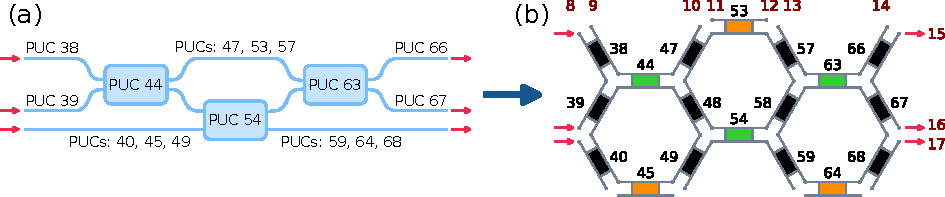
\includegraphics{figures/ch4-mapping_feedforward.pdf}
	\end{center}
	\caption{Mapping between the Clements \cite{clements_optimal_2016} feedforward operator circuit (a) of dimension 3 and its implementation in the hexagonal mesh (b)}\label{fig:ch4-mapping_feedforward}
\end{figure}

The iPronics v1 and v2 meshes can allocate a unitary matrix size of up to 6-by-6.
Obviously smaller unitary operators can be implemented using smaller subsections of the core and larger sizes will have to be split in tiles as needed to fit in this core.
However, the equations derived to map the phases used by a feedforward multi-port interferometer (e.g., Clements or Reck) into the phases to be programmed on a hexagonal waveguide mesh arrangement are agnostic to the matrix size.
Here we summarize the phase equivalence equations obtained for the three different scenarios that can be encountered when implementing such circuits.
Such translation defines a series of phase values that can be used to drive the MZI actuators and then implement the linear matrix multiplication in the hexagonal integrated waveguide array.

\subsection{The feedforward PUC}\label{sub:the_feedforward_puc} % (fold)

The feedforward PUC consists of a single-loaded MZI preceded by a phase shift at one input port.
We can map such structure to our hexagonal mesh by translating the MZI with the phase shifter using a trilattice formed by three PUCs.
Schematically this mapping could be visualized as in Figure~\ref{fig:ch4-mapping_trilattice}.
\begin{enumerate}
	\item Blue PUC: External phase shifter
	\item Orange PUC: Photonic wire
	\item Green PUC: Balanced MZI
\end{enumerate}

\begin{figure}[h!]
	\begin{center}
		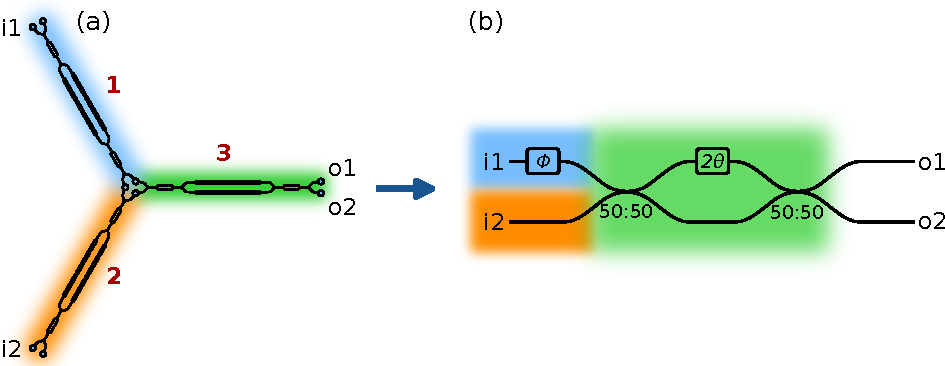
\includegraphics{figures/ch4-mapping_trilattice.pdf}
	\end{center}
	\caption{Mapping of the MZI and the phase shifter in a feedforward mesh (a) using the hexagonal
		architecture (b)}\label{fig:ch4-mapping_trilattice}
\end{figure}

In order for these two structures to have the same behavior, we have to equalize their corresponding transfer function responses so that all the elements match.
On one hand, the matrix representing the FF-PUC is given by \eqref{eq:t_ff}

\begin{equation}
	\label{eq:t_ff}
	T_{FF} = je^{j\frac{\theta}{2}}
	\begin{bmatrix}
		e^{j\phi} sin(\frac{\theta}{2}) & cos(\frac{\theta}{2})  \\
		e^{j\phi} cos(\frac{\theta}{2}) & -sin(\frac{\theta}{2})
	\end{bmatrix}
\end{equation}
where $\phi$ is the external actuator phase and $\theta$ is the PUC's phase shifter value.

On the other hand, the matrix representing the dual-driven PUC present in the hexagonal mesh is given by Equation~\eqref{eq:t_hex}

\begin{equation}
	\label{eq:t_hex}
	T_{H} = je^{j\Delta}
	\begin{bmatrix}
		sin(\theta) & cos(\theta)  \\
		cos(\theta) & -sin(\theta)
	\end{bmatrix}
\end{equation}
where $\Delta = (\phi_{up} + \phi_{lo})/2$ and $\theta = (\phi_{up} - \phi_{lo})/2$.

For the translation we need to make sure that the response of the PUC in Figure~\ref{fig:ch4-mapping_trilattice}(b) is equal to the composite version in (a).
If we address the elements in the matrices in \eqref{eq:t_ff}, \eqref{eq:t_hex} using the $i,j$ subscripts, where
$i$ and $j$ represent the row and column indices of the matrix we can relate the elements in Fig.~\ref{fig:ch4-mapping_trilattice} (a) and (b) by equating

\begin{equation}
	\label{eq:t_ff_hex0}
	T_{10} = T^{1}_{01}T^{3}_{10} \end{equation}

Where the left-hand side corresponds to the feedforward transfer function element and the right-hand side to the hexagonal one.
The upper-scripts refer to the PUC index in Fig.~\ref{fig:ch4-mapping_trilattice}.
Replacing in \eqref{eq:t_ff_hex0} with the corresponding matrix elements for both cases we obtain that

\begin{equation}
	\label{eq:t_ff_hex1}
	je^{j\frac{\theta_{FF}}{2}}cos(\frac{\theta_{FF}}{2})e^{j\phi_{FF}} = (je^{j\Delta^{(1)}_{H}}cos(\theta^{(1)}_{H}))(je^{j\Delta^{(3)}_{H}}cos(\theta^{(3)}_{H}))
\end{equation}

Where the left-hand side corresponds to the feedforward transfer function element and the right-hand side to the hexagonal one.
Solving for $\phi^{(1)}_{up}$, $\phi^{(1)}_{lo}$, $\phi^{(3)}_{up}$ and $\phi^{(3)}_{lo}$ we get

\begin{equation}
	\label{eq:map_ff_hex_1}
	\phi^{(1)}_{up} = \phi^{(1)}_{lo} = \phi_{FF} - \frac{\pi}{2}
\end{equation}

\begin{equation}
	\label{eq:map_ff_hex_2}
	\phi^{(3)}_{up} = \theta_{FF},\; \phi^{(3)}_{lo} = 0
\end{equation}

The equations for PUC\(_2\) in Fig.~\ref{fig:ch4-mapping_trilattice}(a) are obtained by equating

\begin{equation}
	\label{eq:t_ff_hex2}
	T_{11} = T^{2}_{10}T^{3}_{11} \end{equation}

Where the left-hand side corresponds to the feedforward transfer function element and the right-hand side to the hexagonal one.
Replacing in \eqref{eq:t_ff_hex2} with the corresponding matrix elements for both cases we obtain that

\begin{equation}
	\label{eq:t_ff_hex3}
	-je^{j\frac{\theta_{FF}}{2}}sin(\frac{\theta_{FF}}{2}) = (je^{j\Delta^{(2)}_{H}}cos(\theta^{(2)}_{H}))(-je^{j\Delta^{(3)}_{H}}sin(\theta^{(3)}_{H}))
\end{equation}

Solving for $\phi^{(2)}_{up}$, $\phi^{(2)}_{lo}$ one obtains

\begin{equation}
	\label{eq:map_ff_hex_3}
	\phi^{(2)}_{up} = \phi^{(2)}_{lo} = - \frac{\pi}{2}
\end{equation}

Equations~\eqref{eq:map_ff_hex_1}, \eqref{eq:map_ff_hex_2} and \eqref{eq:map_ff_hex_3} represent the generic relations needed to map the phases from a feedforward PUC to its equivalent trilattice in a hexagonal mesh.

% subsection The feedforward PUC (end)
\subsection{Auxiliary edge connections}

When implementing a rectangular feedforward mesh on the hexagonal core we will need to use auxiliary hexagonal PUCs in the edges of the feedforward circuit to connect the trilattice-based PUCs described before.
These connections are presented in Figure~\ref{fig:ch4-pucs_type_a_b}.
Such PUCs were previously described in \cite{perez_silicon_2017} as type A and B, respectively.
For consistency, we will maintain that notation here.

For these pair of PUCs to work as their equivalent in the rectangular implementation (a straight waveguide) we need to equate their combined response to the rectangular equivalent (i.e., a photonic wire) as shown in \eqref{eq:t_ff_hex4} and \eqref{eq:t_ff_hex5}.
We hence obtain for the Type A connection

\begin{equation}
	\label{eq:t_ff_hex4}
	(je^{j\Delta^{(1)}_{H}}cos(\theta^{(1)}_{H}))(-je^{j\Delta^{(2)}_{H}}sin(\theta^{(2)}_{H})) = 1
\end{equation}

thus,

\begin{equation}
	\label{eq:map_ff_hex_a_1}
	\phi^{(1)}_{up} = \phi^{(1)}_{lo} = - \frac{\pi}{2}
\end{equation}

\begin{equation}
	\label{eq:map_ff_hex_a_2}
	\phi^{(2)}_{up} = \pi, \; \phi^{(2)}_{lo} = 0.
\end{equation}

And similarly, for the Type B connection we have

\begin{equation}
	\label{eq:t_ff_hex5}
	(je^{j\Delta^{(1)}_{H}}cos(\theta^{(1)}_{H}))(je^{j\Delta^{(2)}_{H}}sin(\theta^{(2)}_{H})) = 1
\end{equation}

thus,

\begin{equation}
	\label{eq:map_ff_hex_b_1}
	\phi^{(1)}_{up} = \phi^{(1)}_{lo} = - \frac{\pi}{2}
\end{equation}

\begin{equation}
	\label{eq:map_ff_hex_b_2}
	\phi^{(2)}_{up} = 0, \; \phi^{(2)}_{lo} = -\pi.
\end{equation}

\begin{figure}[t]
	\centering
	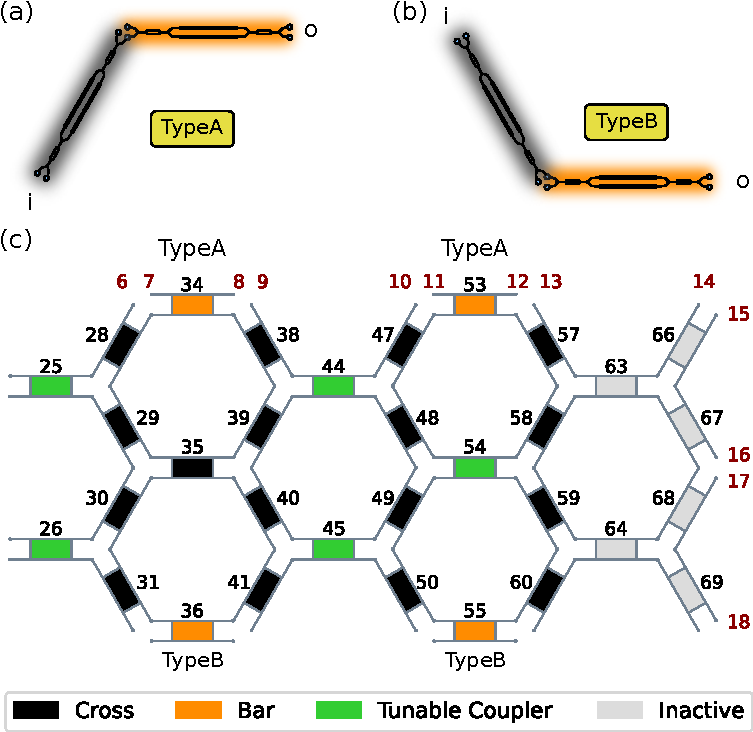
\includegraphics{figures/ch4-pucs_type_a_b.pdf}
	\caption{
		Pairs of PUCs of two types (A and B) allow having a complete implementation of a rectangular mesh on the hexagonal core.
	}\label{fig:ch4-pucs_type_a_b}
\end{figure}

Notice that Equations~\eqref{eq:map_ff_hex_3}, \eqref{eq:map_ff_hex_a_1} and \eqref{eq:map_ff_hex_b_1} are all the same.
This makes sense if we remember that in the three cases the PUCs have to be configured in a cross state without a cross phase to represent a single photonic wire.
Therefore, we can consider \eqref{eq:map_ff_hex_3} to be general for this scenario.

To sum up, if we want to map an arbitrary rectangular architecture to its hexagonal equivalent, we will need to convert the phases obtained using the Clements/Reck decomposition according to the equations presented above.
Equations~\eqref{eq:map_ff_hex_1} and \eqref{eq:map_ff_hex_2} will need to be used for all the MZI phases in the feedforward circuit.
For all the auxiliary PUCs, Equations~\eqref{eq:map_ff_hex_3}, \eqref{eq:map_ff_hex_a_2} and \eqref{eq:map_ff_hex_b_2} need to be used depending on the PUC state and/or the type of connection.

% section Feedforward to Hexagonal translation (end)
\section{Calibration of rectangular feedforward circuit}\label{sec:ff_calibration} % (fold)

Previous publications show that a calibration routine is needed to effectively perform matrix operation on MZI-based unitary operators \cite{alexiev_calibrating_2021}.
Although the hexagonal meshes, subject of this work, have already gone through the calibration process covered in Section~\ref{sub:calibration}, this process only took into account the parasitic phases between the PUC arms.
However, in the case of circuits like the Clements circuit, another set of passive phases must be taken into account: the interconnection between PUCs.
The results previously published in \cite{perez-lopez_general-purpose_2024, on_programmable_2024} already pointed that whenever a recirculating interferometric structure was implemented on the hexagonal arrays a phase mismatch could be deduced from their spectral response.
The study of these occurrences led us to the proposal of a new non-ideal model for a PUC that can account for this and can be used as a basis for a complementary calibration routine for such structures.

\subsection{Updated PUC model}\label{sub:updated_puc_model} % (fold)

\begin{figure}[t]
	\begin{center}
		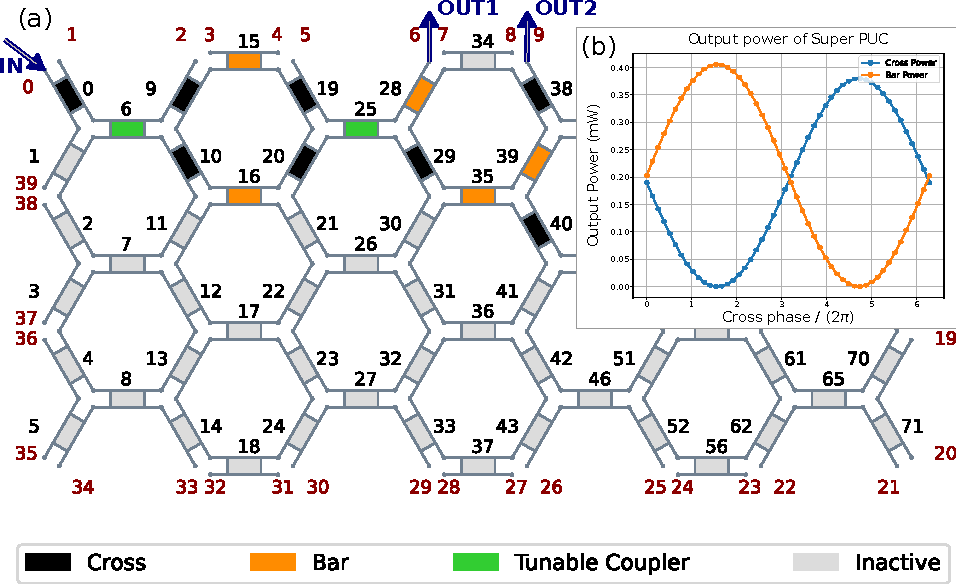
\includegraphics{figures/ch4-superpuc.pdf}
	\end{center}
	\caption{MZI instantiated in the hexagonal mesh (left) and its measured output power for different cavity
		phases}\label{fig:ch4-superpuc}
\end{figure}

To understand the effect of parasitic interconnection phases in hexagonal cells we start by studying the simplest case: the balanced MZI circuit, i.e., a circuit composed by the 6 PUCs surrounding a hexagonal cell as presented in Figure~\ref{fig:ch4-superpuc}.
The phase difference between the upper and lower arms of this MZI should in theory be zero and therefore the MZI circuit should be in cross state by default.
As covered in Section~\ref{sub:calibration}, using \lstinline|set_coupling_factor_phase|, each composing PUC can be programmed to a have a 0 cross-phase, therefore the compound circuit should behave as an ideal MZI.
However, what we observe in Figure~\ref{fig:ch4-superpuc} is that the circuit is configured as if an effective phase shift had been applied to one of its arms when that's not the case.
This led us to conclude that a parasitic phase shift is introduced at the chip level.
The same behavior has been reported in other structures such as rings and filters.

\begin{figure}
	\begin{center}
		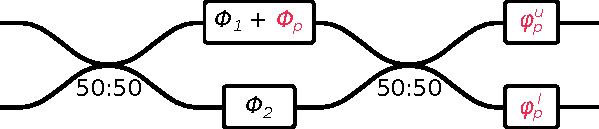
\includegraphics{figures/ch4-pucmodel.pdf}
	\end{center}
	\caption{Proposed new model of non-ideal PUC}\label{fig:ch4-pucmodel}
\end{figure}

To better explain this phenomenon we have proposed the new non-ideal PUC model depicted in Figure~\ref{fig:ch4-pucmodel}.
In addition to the internal passive phase shift within the PUC arms we now also consider the shift introduced by the silicon waveguide interconnections between PUCs.
The effects of these spurious phases are clearly observed in phase-dependent circuits such as filters, interferometric operators but are also completely masked by the photodetectors in amplitude-only applications such as switches and beamsplitters.
Therefore, for coherent applications we must perform an additional calibration routine.
To sum up, the routine in Section~\ref{sub:calibration_of_puc_cells} compensates \(\phi_p\) within the PUC and the passive phases between PUCs \(\phi^u_p\) and \(\phi^l_p\) must be characterized using an additional routine.

% subsection Updated PUC model (end)
\subsection{Calibration of PUC cells}\label{sub:calibration_of_puc_cells} % (fold)

Finding out the values of \(\phi^u_p\) and \(\phi^l_p\) for the entire mesh is a nontrivial task and a discussion of its possible acquisition has been reserved for Section~\ref{sub:circuit_aware_calibration}.
Here we limit our study to a lumped element simplification that can be used for the case of multi-port interferometers.
Considering the phase introduced in the connection between PUCs we know that the phases introduced in the lower and upper arms are not the same.
The experimental results indicate that the phase difference between the arms is not zero.
Following the new PUC model we can express this parasitic phase difference this way:
\begin{equation}
	\phi^l_{up} = \phi^{(6,9)} + \phi^{(9,15)} + \phi^{(15,19)} + \phi^{(19,25)}
	\label{eq:ch4-superpuc_up}
\end{equation}

\begin{equation}
	\phi^l_{lo} = \phi^{(6,10)} + \phi^{(10,16)} + \phi^{(16,20)} + \phi^{(20,26)}
	\label{eq:ch4-superpuc_lo}
\end{equation}
where \eqref{eq:ch4-superpuc_up} and \eqref{eq:ch4-superpuc_lo} correspond to the total lumped (\(l\)) parasitic phase on each arm, respectively.
Therefore, to calibrate this MZI circuit, we need to compensate the equivalent lumped circuit phase \(\phi^l_{MZI}\) \eqref{eq:ch4-superpuc_lumped} given by the difference between upper and lower arms:

\begin{equation}
	\phi^l_{MZI} = \phi^l_{up} - \phi^l_{lo}.
	\label{eq:ch4-superpuc_lumped}
\end{equation}

This means that if we want to calibrate an MZI circuit we need to apply \(-\phi^l_{MZI}\) as a compensation cross-phase to a PUC in the upper arm of the cell.
Note that, as shown in Figure~\ref{fig:ch4-superpuc_hex}, the use the lumped model simplification removes the need to characterize the values \(\phi^u_p\) and \(\phi^l_p\) of each PUC.
If From here onwards we will drop the \(l\) superscript and consider all parasitic phases lumped unless otherwise stated.
This phase value must be compensated for each cell in the mesh so that a synthesized MZI circuit will be set to cross state.
Therefore, in hardware, to find the compensating phase, we use a gradient descent optimizer \cite{noauthor_optimization_nodate} to find the phase that maximizes the cross power.
We use an optimizer instead of a phase sweep as it converged more quickly on the right calibration phase and this time we don't need to characterize the full MZI response as reported in Section~\ref{sub:calibration}.
This phase could then be added to any PUC that forms the upper/lower arms.
The process was then automated and repeated for all the cells in the mesh (see Figure~\ref{fig:ch4-hex_cells}).

\begin{figure}[h]
	\begin{center}
		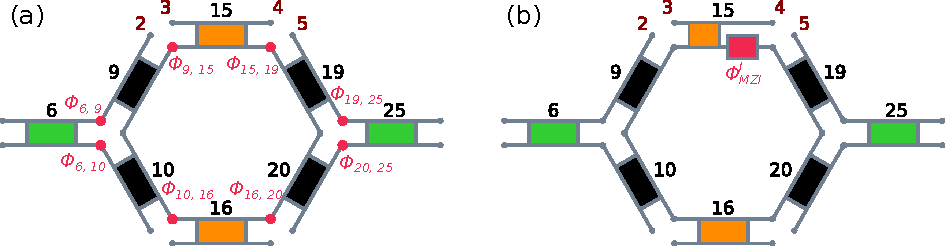
\includegraphics{figures/ch4-super_puc_hex.pdf}
	\end{center}
	\caption{Non-ideal junction phases added to hexagonal cells (a) and their corresponding lumped model (b)}\label{fig:ch4-superpuc_hex}
\end{figure}

\begin{figure}
	\begin{center}
		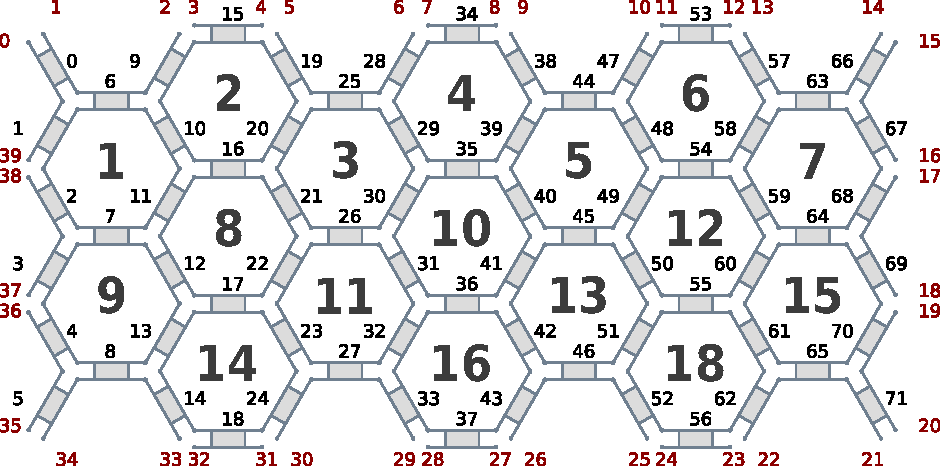
\includegraphics{figures/ch4-hex_cells.pdf}
	\end{center}
	\caption{Numbered MZI cells in the iPronics hexagonal core}\label{fig:ch4-hex_cells}
\end{figure}

% subsection Calibration of PUC cells (end)

\subsection{Calibration of feedforward operators}\label{sub:calibration_of_feedforward_operators} % (fold)

\begin{figure}
	\begin{center}
		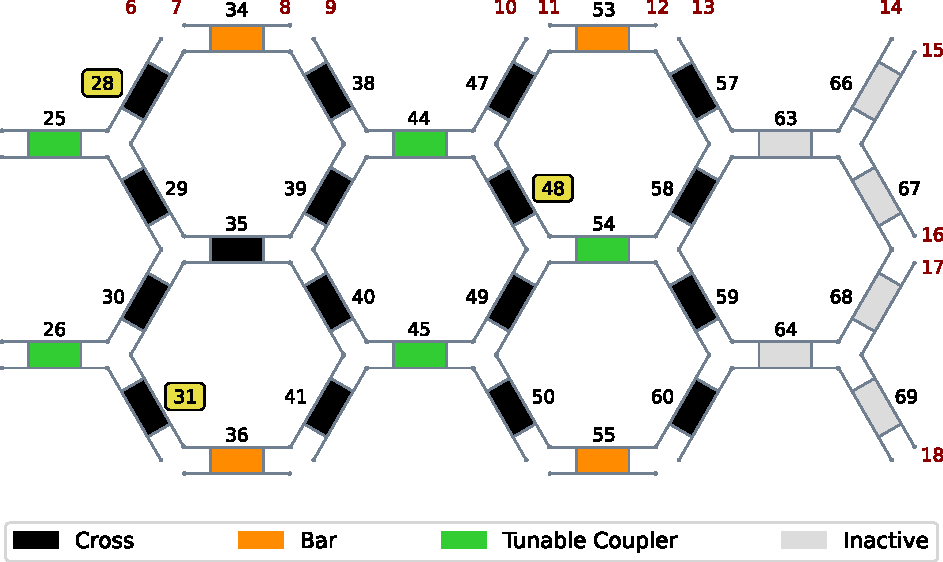
\includegraphics{figures/ch4-superpuc_compensation.pdf}
	\end{center}
	\caption{Synthesized feedforward mesh with PUCs where the compensation is applied as a cross-phase delta
		(yellow)}\label{fig:ch4-superpuc_compensation}
\end{figure}

The calibration presented in Section~\ref{sub:calibration_of_puc_cells} corrects the lumped passive phase inside each MZI circuit.
To calibrate the multiport interferometer (i.e., the Clements mesh), we can use the phases obtained from the previous MZI calibration.
In this kind of feedforward mesh the cavities are coupled so that we should be careful when choosing where we compensate the passive phases of each individual MZI.
The most effective way to do that is to compensate the phases in PUCs that are not shared between hexagonal cavities.
For example, in Figure~\ref{fig:ch4-superpuc_compensation} to calibrate a 4-port unitary operator we can apply the compensation phases to PUCs 28, 31 and 48 to calibrate the MZIs placed on hex cells 4, 10 and 5, respectively (refer to Fig.~\ref{fig:ch4-hex_cells}).
There might be scenarios for which isolated compensation is not possible.
In those cases we can compensate the cells taking into account the overlap between paths.
For example, suppose we are restricted to compensate with PUCs 35, 40 and 49 (chosen for illustrative purposes).
In this scenario the phases applied to calibrate the whole Clements circuit are
\begin{equation}
	\begin{aligned}
		\phi^{(35)} & = -\phi^{(4)}_{MZI}                                        \\
		\phi^{(40)} & = \phi^{(10)}_{MZI} + \phi^{(4)}_{MZI}                     \\
		\phi^{(49)} & = -\phi^{(5)}_{MZI} - \phi^{(10)}_{MZI} - \phi^{(4)}_{MZI}
	\end{aligned}
	\label{eq:ch4-clements_calib_complex}
\end{equation}
where the phases on the left-hand side correspond to the effective cross-phase applied to an individual PUC and the phases on the right-hand side correspond to each MZI cell parasitic phase.
With these calibration phases, the feedforward circuit's phase response will now be error free.

% subsection Calibration of feedforward operators (end)
% section Calibration of synthesized feedforward circuit (end)

\section{Feedforward operator}\label{sec:feedforward_operator} % (fold)

\subsection{Feedforward operator in code}\label{sub:feedforward_operator_in_code} % (fold)

\begin{lstlisting}[caption={A 3x3 Feedforward operator instance in hexagonal mesh}, label={lst:ch4-definition}]
	feedforward = smart.feedforward_operator(dim=3, puc_0=0)
	smart.load_feedforward_config(feedforward)
	core_monitor.plot_mesh_status()
\end{lstlisting}

Once these calibration phases have been loaded to the feedforward operator circuit, the equivalent Hexagonal-Clements decomposition phases presented in Section~\ref{sec:feedforward_to_hexagonal_translation} can be applied to the circuit PUCs.
Here we cover the implementation of such operator as a logical element that can be synthesized on the first-generation Smartlight hexagonal core through a simple set of Python instructions.
Listing~\ref{lst:ch4-definition} shows the instructions needed to instantiate a logical feedforward circuit.
First, we generate the feedforward operator object using \lstinline|feedforward_operator(dim, puc_0)|.
By specifying the input parameter \lstinline|dim|, we have flexibility to select the dimension of our feedforward operator.
Given the specifications of the first-generation Smartlight mesh, we are capable of creating feedforward operators with dimensions ranging from 2 to 6.
Moreover, we can also choose where to place the feedforward operator through the \lstinline|puc_0| parameter.
This location is indicated with the PUC in the upper left corner of the operator, in which the lower port is the one used to input the signal.
After creating the operator object, one can integrate it into the mesh by employing \lstinline|load_feedforward_config()| and providing the previously generated operator as the input parameter.

\begin{figure}
	\begin{center}
		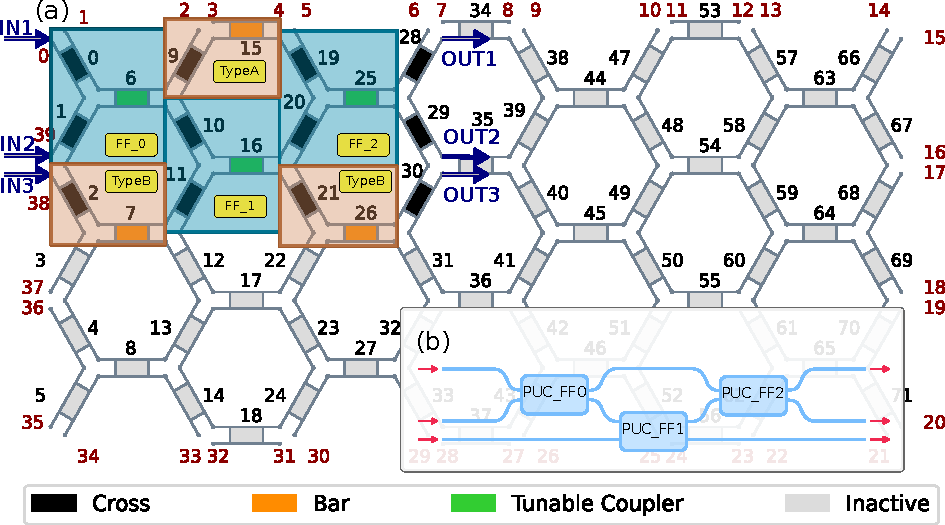
\includegraphics{figures/ch4-ff_in_hex.pdf}
	\end{center}
	\caption{(a) A 3-by-3 Feedforward operator instance with all its compoosing elements implemented in the hexagonal mesh. (b) equivalent Clements circuit of size \(N=3\).}\label{fig:ch4-ff_in_hex}
\end{figure}

We can always access to the feedforward operator created using the \lstinline|puc_config| attribute as shown in Listing~\ref{lst:ch4-puc-translation}.
As we have seen in previous sections, the configuration of each PUC can be provided by two distinct methods:

\begin{enumerate}
	\item \lstinline|set_coupling_factor_phase()|: Sets a coupling factor $k$ and a cross phase $\Delta$
	\item  \lstinline|set_driven_phases()|: Sets directly the phases $\phi_{lo}$ and $\phi_{up}$
\end{enumerate}

In this case, we will use the second option to load the phases derived in Section~\ref{sec:feedforward_to_hexagonal_translation}.
As explained in that section, a trilattice is conformed by three PUCs with different behaviors: a tunable coupler, a phase shifter and a photonic wire.
Therefore, each instance of \lstinline|FeedForwardOperator| is associated with three sets of PUCs, each with their respective functionalities as shown in Listing~\ref{lst:ch4-puc-translation} and Figure~\ref{fig:ch4-ff_in_hex}.

\begin{lstlisting}[caption={Equivalence between hexagonal PUCs and feedforward ones},
label={lst:ch4-puc-translation}]
	# Access to the puc configuration
	puc_config = feedforward.puc_config
	# Consult which PUCs are tunable couplers
	tunable_couplers = feedforward.coupler_pucs
	# Consult which PUCs are tunable phase shifters
	phase_shifters = feedforward.phase_shifters
	print("PUCs acting as tunable coupler are:", tunable_couplers)
	>>> PUCs acting as tunable coupler are: [6, 16, 25]
	print("PUCs acting as phase shifter are:", phase_shifters)
	>>> PUCs acting as phase shifter are: [0, 10, 19]
\end{lstlisting}

% subsection Feedforward operator in code (end)
\subsection{Implementation of arbitrary unitary matrices}\label{sub:implementation_of_arbitrary_unitary_matrices} % (fold)

%%%%%% puo paper
Based on the aforementioned rationale, we have implemented these operators as logical parametric units that can be placed on different positions of the first-generation Smartlight's mesh \cite{perez-lopez_general-purpose_2024}.
Listing~\ref{lst:ch4-instruction} presents the instruction set we have developed to instantiate unitary operators on a hexagonal-based chip architecture.
The parametric and floating nature of the operator is presented in line 3, where the developer inputs the dimension \lstinline|N| of the logical unit and its location \lstinline|puc_0| on the hexagonal grid, respectively.
The dimensions of the hexagonal mesh constrain both parameters.
The current chip architecture can support operators up to a maximum size of $N = 6$.
The instruction set, however, is agnostic of this constraint and supports larger and smaller meshes.
Line 5 shows how a unitary matrix $U$ is loaded to the chip.
This instruction performs the mathematical decomposition and translation from Clements-based phases to their hexagonal equivalent.
Line 7 then loads this new phase configuration on the logical operator, considering calibration data from its location on the hexagonal grid, to end up with the unitary implemented on hardware.
By following this procedure, logical unitary operators can be deployed on different mesh locations and be accessed through the system I/O ports or connected to other subcircuits on the mesh in a place-and-route fashion for further application development.
Note that because of this floating feature any of the mesh I/O ports or the internal mesh node can be used as inputs to the parametric unitary operator.

\begin{lstlisting}[caption={Basic instruction set needed to implement matrix operators on the first-generation Smartlight}, label={lst:ch4-instruction}]
	from smartlight import feedforward_operator
	# Create operator
	ff = feedforward_operator(dim=N, puc_0=38)
	# Load matrix to the operator
	ff.load_unitary_matrix(U)
	# Load phase configuration into the mesh
	hex_mesh.load_feedforward_config(ff)
\end{lstlisting}

To illustrate this procedure, let's review the implementation of a 1-by-3 beamsplitter.
First, we define the transfer matrix presented in Eq.~\eqref{eq:beamsplitter}

\begin{equation}
	\label{eq:beamsplitter}
	T_{BS} = \frac{1}{\sqrt{3}} \begin{bmatrix}
		1 & 1            & -1          \\
		1 & e^{i2\pi/3}  & e^{i4\pi/3} \\
		1 & e^{-i4\pi/3} & e^{i8\pi/3}
	\end{bmatrix}
\end{equation}

With \(I = \begin{bmatrix} 1 & 0 & 0 \end{bmatrix}^T\) acting as normalized input for this particular case in which the internal laser (\(P=5\)~dBm) is connected to the first unitary operator port.
Eq.~\eqref{eq:beamsplitter} is implemented in hardware using the code in Listing~\ref{lst:ch4-beamsplitter}.

\begin{lstlisting}[caption={Implementation of a three-way beamsplitter using a Feedforward operator},
label={lst:ch4-beamsplitter}]
	# T_BS: Transfer matrix of a 1-by-3 beamsplitter
	smart.reset_mesh()
	# Create the feedforward operator
	feedforward = smart.feedforward_operator(dim=3, puc_0=38)
	feedforward.load_unitary_matrix(T_BS)
	# Load the feedforward configuration into the mesh
	smart.load_feedforward_config(feedforward)
	# Define input path to operator
	path = [
		(0, ["x", 0]),
		(6, ["=", 0]),
		(9, ["x", 0]),
		(15, ["=", 0]),
		(19, ["x", 0]),
		(25, ["=", 0]),
		(28, ["x", 0]),
		(34, ["=", 0]),
	]
	smart.set_coupling_factor_phase(path)
	core_monitor.plot_mesh_status()
\end{lstlisting}

\begin{figure}
	\begin{center}
		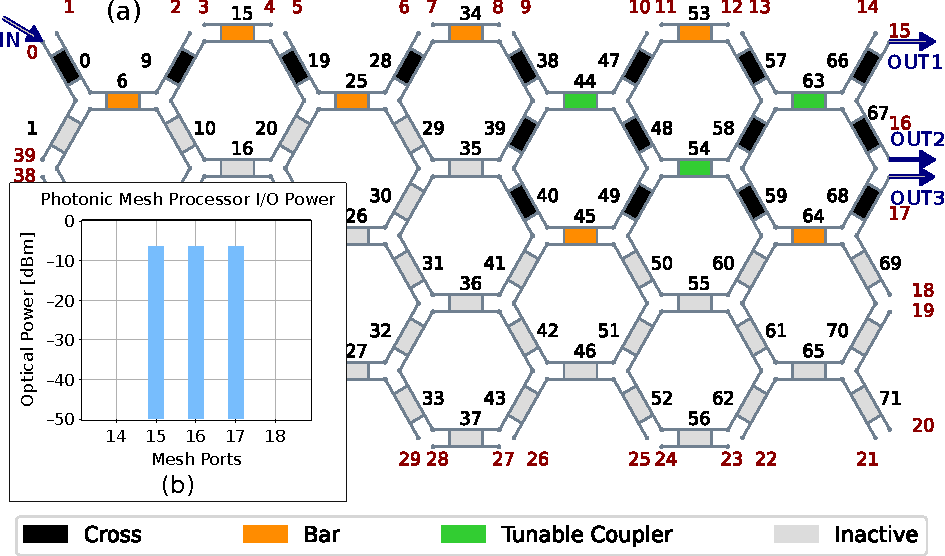
\includegraphics{figures/ch4-3split_mema.pdf}
	\end{center}
	\caption{(a) Implementation of three-way beamsplitter in the hexagonal mesh using a 3-by-3  Feedforward
		operator.
		In (b) the output power distribution observed by the MEMA monitor.
	}\label{fig:ch4-3split} \end{figure}

The resulting circuit is presented in Figure~\ref{fig:ch4-3split}, where one can observe the unitary operator spanning from PUC 38 and with its outputs directly connected to the mesh output ports for power monitoring.
Additionally, an optical interconnect has been created to connect one input of the operator to the laser at system port 0.
By plotting the output distribution using the power monitor, we can see that the power has been equally distributed among the three outputs with a split of -4.77 dB corresponding to \(\frac{1}{3}\) (see Figure~\ref{fig:ch4-3split}(b)).

In the following section, we conclude this chapter by covering some applications of interest for the telecom/datacom community involving unitary operators of different sizes.
% subsection Implementation of arbitrary unitary matrices (end)
%-------------------------------------------------- Hybrids Section -------------------------------------------------------%
\section{Optical hybrids for coherent links}
% - 'Experiment explanation':
% - Matrix Equations
\begin{figure}[t!]
	\centering
	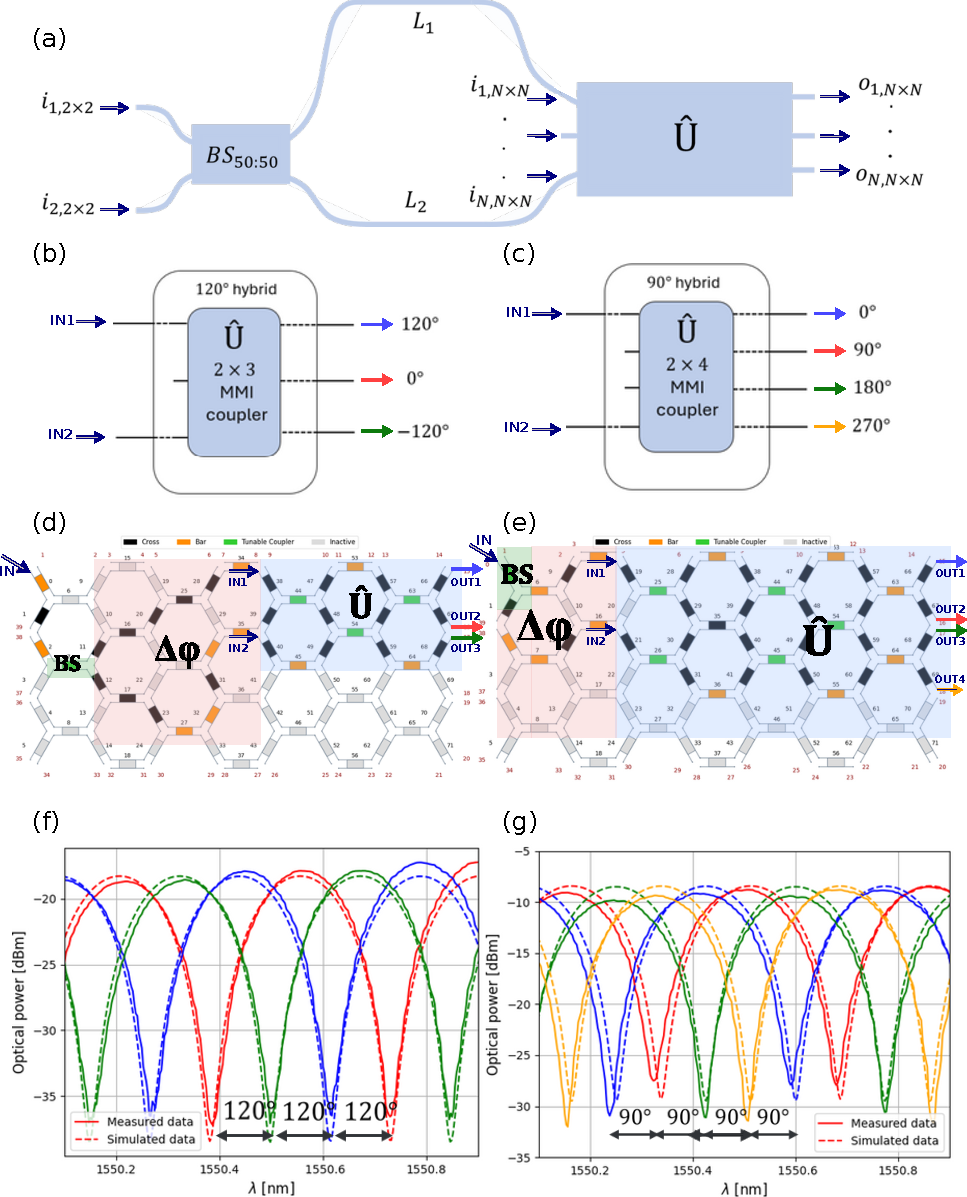
\includegraphics{figures/ch4-hybrids.pdf}
	\caption{Photonic circuit (a) used to demonstrate the 120$^o$ (b) and 90$^o$ (c) hybrid functionality of a logical unitary operator synthesized on hexagonal chip architecture (d-e).
		Optical power measured at the operators' outputs, shown in different colors, for the 120$^o$ (f) and 90$^o$ (g) hybrids with their resulting phase difference inferred from the FSR.
	}
	\label{fig:hybrids}
\end{figure}

Coherent transceivers are ubiquitous elements of telecom links.
Their use within data centers has only been limited by the lower price and power consumption of their intensity-modulation direct-detection (IM-DD) counterparts.
The progressive introduction of coherent technology in data centers is predicted to grow during the next decade to satisfy data rate increasing demands.
\cite{maharry_first_2022}.
A key element of these devices on the reception side is a hybrid capable of mixing the incoming signal with the local oscillator (LO) and producing a combined output with both signals out of phase by a certain $\Delta\phi$ angle between them.
The mathematical representation of this operation is given by Eq.~\eqref{eq:mmi3} for 120$^o$ and Eq.~\eqref{eq:mmi4} for 90$^o$, which in turn corresponds to the transfer functions of 3x3 and 4x4 MMIs, respectively.
\begin{equation}\label{eq:mmi3}
	U = \frac{1}{\sqrt{3}}
	\begin{bmatrix}
		-e^{-i2\pi/3} & e^{-i2\pi/3} & -1             \\
		e^{-i2\pi/3}  & -1           & e^{-i2\pi/3}   \\
		-1            & e^{-i2\pi/3} & - e^{-i2\pi/3}
	\end{bmatrix}
\end{equation}

\begin{equation}\label{eq:mmi4}
	U = \frac{1}{\sqrt{4}}
	\begin{bmatrix}
		e^{i\pi}    & e^{-i\pi/4} & e^{i3\pi/4} & e^{i\pi}    \\
		e^{-i\pi/4} & e^{i\pi}    & e^{i\pi}    & e^{i3\pi/4} \\
		e^{i3\pi/4} & e^{i\pi}    & e^{i\pi}    & e^{i7\pi/4} \\
		e^{i\pi}    & e^{i3\pi/4} & e^{i7\pi/4} & e^{i\pi}    \\
	\end{bmatrix}
\end{equation}
Since Equations~\eqref{eq:mmi3}, \eqref{eq:mmi4} refer to linear systems, they can easily be implemented on a hexagonal mesh using the logical unitary operator introduced in the previous section.
To demonstrate the hybrid operation, the circuit in Fig.~\ref{fig:hybrids}(a) is synthesized on the mesh.
Here, the injected light is split using a 3-dB coupler, and an asymmetric MZI structure is connected to the hybrid's input.
Insets (b) and (d) show the implementation when the operator tested is a 120$^o$ hybrid ($U = $ Eq.~\eqref{eq:mmi3}), and insets (c) and (e) show the 90$^o$ case ($U = $Eq.~\eqref{eq:mmi4}).
In (f) and (g), we observe the power measured at the outputs of the operator for the two cases.
The relative phase differences are determined using the $\Delta\phi/\Delta\lambda = 2\pi/FSR$.
The solid lines represent the experimental results, and the dotted ones are the simulated ones.
These traces closely match each other and replicate the ones of previously reported dedicated 120$^o$ and 90$^o$ hybrids \cite{saber_demonstration_2018, yu_high-performance_2020, reyes-iglesias_high-performance_2012}, thus demonstrating that the operator can deploy both functionalities using the same hardware.

%-------------------------------------------------- Multicast Section -------------------------------------------------------%
\section{The WDM multicast switch}

%- Matrix Equations
%- Experiment explanation
%- Application in WDM links

Multicast switches (MCS) are key elements of existing ROADM solutions in which the combination of wavelength selective switches (WSS), tunable filters, and optical amplifiers alongside the MCS enable the so-called colorless, directionless, and contentionless (CDC) operation to meet current internet requirements \cite{watanabe_multicast_2014,yang_low-cost_2017}.
The MCS performs the split and combines operations of different wavelength-carrier signals as shown in Fig.~\ref{fig:multicast}(a).
This linear operation can be represented by Eq.~\eqref{eq:dft}, which corresponds to a DFT operator.
Since the inputs to the operator have different wavelengths, the DFT phase shifts don't have any effect, and $U$ acts as a split-and-combine operator.

\begin{equation}\label{eq:dft}
	U = \frac{1}{\sqrt{6}}
	\begin{bmatrix}
		1 & 1           & 1           & 1  & 1           & 1           \\
		1 & e^{i\pi/3}  & e^{2i\pi/3} & -1 & e^{i4\pi/3} & e^{i5\pi/3} \\
		1 & e^{2i\pi/3} & e^{i4\pi/3} & 1  & e^{i2\pi/3} & e^{i4\pi/3} \\
		1 & -1          & 1           & -1 & 1           & -1          \\
		1 & e^{i4\pi/3} & e^{2i\pi/3} & 1  & e^{i4\pi/3} & e^{i2\pi/3} \\
		1 & e^{i5\pi/3} & e^{i4\pi/3} & -1 & e^{i2\pi/3} & e^{i\pi/3}  \\
	\end{bmatrix}
\end{equation}

To test this operation mode, we have created an $N=6$ logical operator, loaded the DFT matrix to it, and connected its inputs to six lasers with different wavelengths, see Fig.~\ref{fig:multicast}(b).
As seen by a spectrum analyzer, the output from this system is shown in (c), where the spectra of the six input carriers are shown next to the spectrum of output 1.
The latter contains a signal with all six wavelength components combined and powers of -7.78~dB (i.e., a $1/6$ split) with respect to the input laser peak powers, as expected in a practical MCS system.
Note that since this operator implements \eqref{eq:dft} it could also be used to demonstrate the costly DFT operation if same-wavelength inputs and coherent detection were used.

\begin{figure}[h]
	\centering
	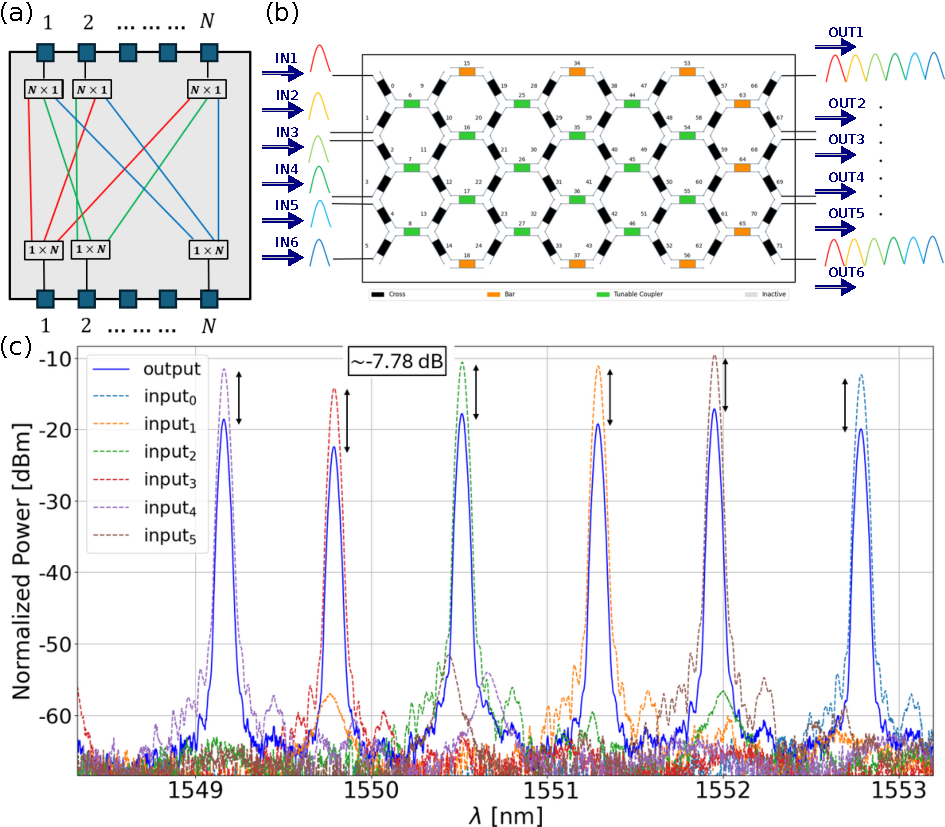
\includegraphics{figures/ch4-mcs.pdf}
	\caption{Schematic (a) of a multicast switch used in ROADMs to split and combine different wavelength carriers and its implementation on the reconfigurable mesh (b) using a 6-by-6 unitary operator.
		The measured spectra in (c) contain the resulting split-and-mixed signal at output port 1-6 and the incoming carriers (other colors).
	}
	\label{fig:multicast}
\end{figure}

%-------------------------------------------------- OCS Section -------------------------------------------------------%
%\section{Optical circuit switching}
%- Matrix Equations
%Eq.~\eqref{eq:switch}

%\begin{equation}\label{eq:switch}
%U=
%\begin{bmatrix}
%0 & 0 & 0  & 1 & 0 & 0 \\
%0 & 0 & 0  & 0 & 1 & 0 \\
%0 & 0 & 0  & 1 & 0 & 1 \\
%1 & 0 & 0  & 0 & 0 & 0 \\
%0 & 1 & 0  & 0 & 0 & 0 \\
%0 & 0 & 1  & 0 & 0 & 0 \\
%\end{bmatrix}
%\end{equation}
%- Experiment explanation
%- Application in DC links

%\lipsum[3]  
%-------------------------------------------------- Conclusions Section -------------------------------------------------------%
\section{Conclusions}
This chapter has introduced the concept of logical unitary operators that can be deployed on a reconfigurable hexagonal chip architecture using a place and route fashion as sub circuits or standalone elements using a short set of code instructions.
We have explored and experimentally demonstrated different applications of such operators using the iPronics first-generation Smartlight platform, including optical hybrids for coherent transceivers and a multicast switch for ROADMs, using different operator sizes.
The applications, however, are far more extensive than this small subset, as linear operations lie at the heart of several optical systems.
With this contribution, we aim to provide the photonics community with a tool that enables and fosters the fast development and deployment of new optical solutions, effectively and flexibly addressing the critical need for innovative, reconfigurable, and mass-manufacturable semiconductor solutions that can fulfil the growing demand for faster and cheaper data transmission.
% section Feedforward operator (end)
% chapter Universal Unitary Operators (end)

